\chapter*{События с группами мюонов в детекторе ДЕКОР}
\addcontentsline{toc}{chapter}{События с группами мюонов в детекторе ДЕКОР}
\label{ch:intro}
Стандартный отбор и анализ групп мюонов по данным детектора ДЕКОР проводится для множественностей мюонов в группе \(m \geq 5\) и зенитных углов \(\theta \geq 55\degree\), чтобы исключить возможное влияние электронно-фотонной и адронной компонент ШАЛ на реконструкцию треков. Однако из части экспериментального материала в интервале зенитных углов \(40\degree \leq \theta < 55\degree\) (вследствие резкого увеличения статистики с уменьшением зенитного угла) операторами ЭК НЕВОД было отобрано 30 375 групп с множественностью мюонов \(m \leq 5\) (за 6 324 ч) и 4 139 групп с множественностью \(m = 4\) (за 1 043 ч). В этом случае установка НЕВОД-ШАЛ в принципе еще должна быть способна регистрировать электронно-фотонную компоненту ШАЛ, что позволяет провести анализ указанных событий совместно как минимум по двум компонентам ШАЛ. Отметим также, что события с группами мюонов отбирались в двух \(60\degree\) секторах азимутальных углов, где шесть из восьми СМ детектора ДЕКОР экранированы водным объемом детектора НЕВОД, причем во внимание принимаются данные только этих шести СМ. Пороговая энергия мюонов при этом составляет около 2 ГэВ. 

Отбор событий с умеренными зенитными углами проводился по 12-й серии измерений из наборов данных (RUN) 622-688 (с 15.02.18 по 29.05.18 г.) и 810-841 (с 13.12.18 по 03.02.19 г.). На рис. 3 изображен пример события с группой мюонов, зарегистрированного установкой ДЕКОР (a) и пространственной реконструкции треков (б).
\newpage
\noindent 19-12-2018 03:02:35.298.921.862, RUN \(=813\),  Event \(=73818\),\\
\(m = 9\), \(\theta = 41.9\degree\), \(\phi=204.9\degree\)

\begin{figure}[ht]
    \centering
    \subfloat[]{%
        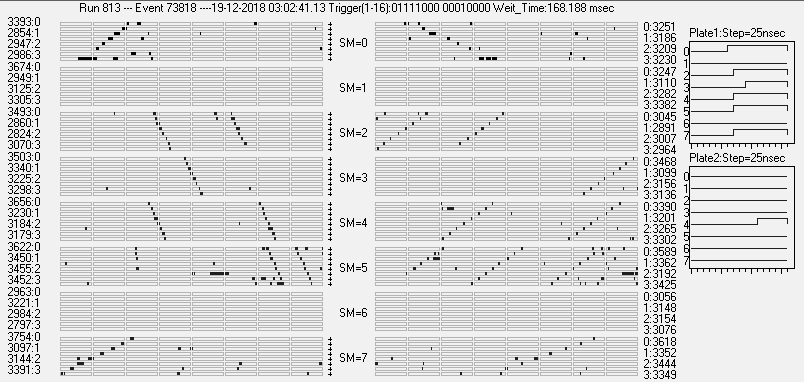
\includegraphics[width=0.95\textwidth, keepaspectratio]{images/73818_1_bw.png}%
        \label{fig:muon_group1}%
    }%

    \subfloat[]{%
        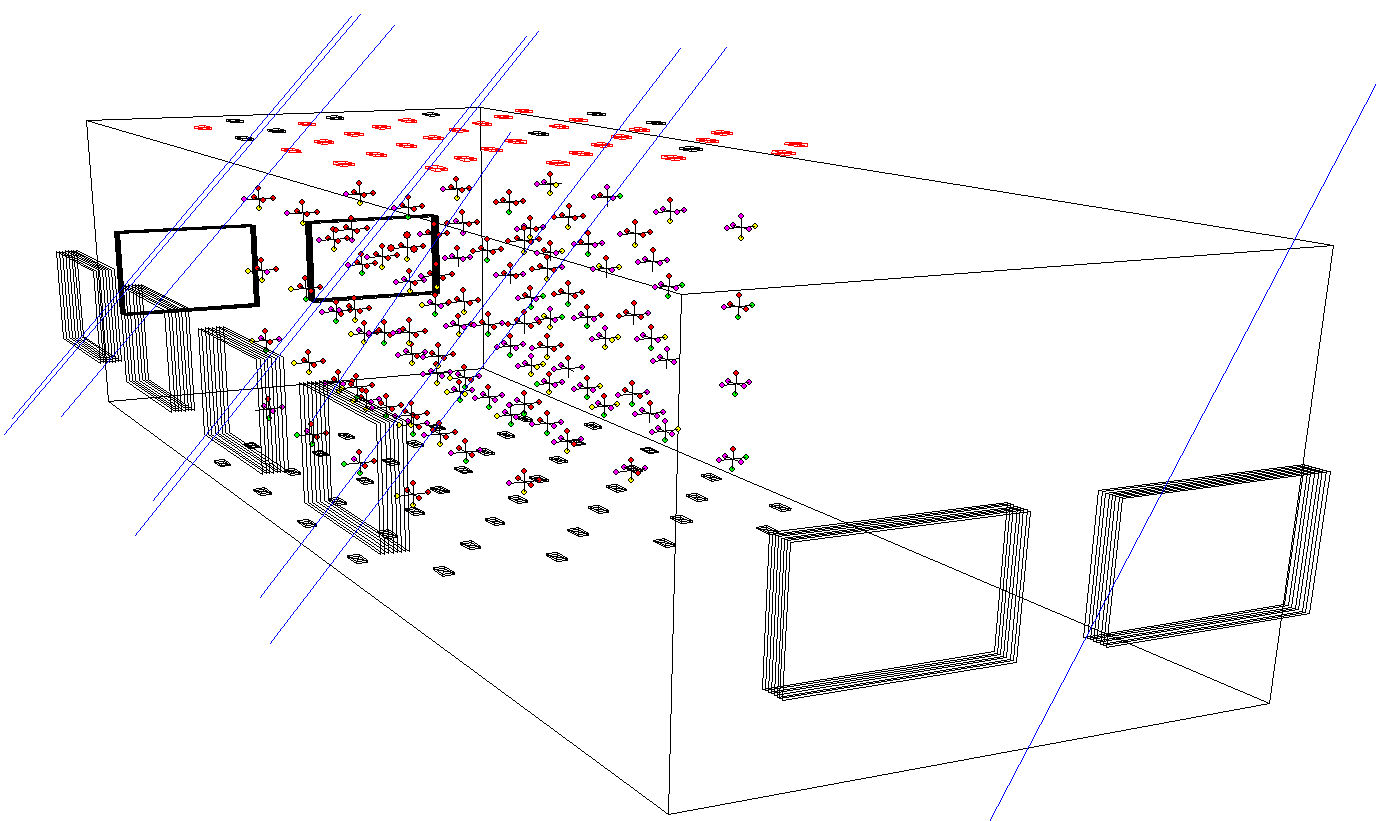
\includegraphics[width=0.95\textwidth, keepaspectratio]{images/73818.png}%
        \label{fig:muon_group}%
    }%

    \caption{Пример события с группой мюонов, зарегистрированного установкой \\ДЕКОР (a) и пространственной реконструкции треков (б)}
    \label{fig:muon_example}
\end{figure}

\newpage
На рисунке 4 представлено распределение зенитного \(\theta\) и азимутального \(\phi\) углов направления прихода 6990 отобранных групп мюонов 810-841 RUN

\begin{figure}[ht]
    \lefting
    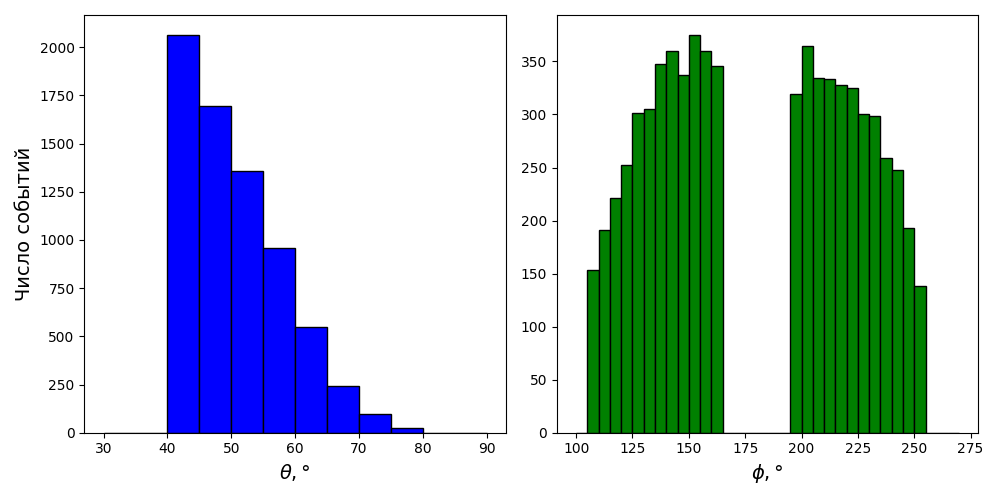
\includegraphics[width=1\textwidth]{images/theta_phi.png}
    \caption{Распределение числа событий с группами мюонов по зенитному\(\theta\) и азимутальному \(\phi\) углу направления прихода}
    \label{fig:phi_hist}
\end{figure}

\endinput